\documentclass[final,hyperref={pdfpagelabels=false}]{beamer}
\usepackage{grffile}
\mode<presentation>{\usepackage{../themes/beamerthemePersyval}}
\usepackage[english]{babel}
\usepackage[latin1, utf8]{inputenc}
\usepackage{amsmath,amsthm, amssymb, latexsym}
%\usepackage{times}\usefonttheme{professionalfonts}  % obsolete
%\usefonttheme[onlymath]{serif}
\boldmath
\usepackage[orientation=portrait,size=a0,scale=1.4,debug]{beamerposter}
% change list indention level
% \setdefaultleftmargin{3em}{}{}{}{}{}


%\usepackage{snapshot} % will write a .dep file with all dependencies, allows for easy bundling

\usepackage{array,booktabs,tabularx}
\newcolumntype{Z}{>{\centering\arraybackslash}X} % centered tabularx columns
%\newcommand{\pphantom}{\textcolor{ta3aluminium}} % phantom introduces a vertical space in p formatted table columns??!!

\listfiles

%%%%%%%%%%%%%%%%%%%%%%%%%%%%%%%%%%%%%%%%%%%%%%%%%%%%%%%%%%%%%%%%%%%%%%%%%%%%%%%%%%%%%%
\graphicspath{{../img/}}

\title{Eye-tracking and electroencephalogram data analysis using hidden Markov models to identify reading strategies}
\author{Brice Olivier\textsuperscript{1,2}, Jean-Baptiste Durand\textsuperscript{1,2}, Anne Guérin-Dugué\textsuperscript{3}, Marianne Clausel\textsuperscript{2}}
\institute{\textsuperscript{1}Inria, \textsuperscript{2}Laboratoire Jean Kuntzmann, \textsuperscript{3}Gipsa-lab}
\date[June 13rd-14th, 2017]{June 13rd-14th, 2017}


%%%%%%%%%%%%%%%%%%%%%%%%%%%%%%%%%%%%%%%%%%%%%%%%%%%%%%%%%%%%%%%%%%%%%%%%%%%%%%%%%%%%%%
\newlength{\columnheight}
\setlength{\columnheight}{105cm}


%%%%%%%%%%%%%%%%%%%%%%%%%%%%%%%%%%%%%%%%%%%%%%%%%%%%%%%%%%%%%%%%%%%%%%%%%%%%%%%%%%%%%%
\begin{document}
\begin{frame}
  \begin{columns}
    % ---------------------------------------------------------%
    % Set up a column
    \begin{column}{.49\textwidth}
      \begin{beamercolorbox}[center,wd=\textwidth]{postercolumn}
        \begin{minipage}[T]{.95\textwidth}  % tweaks the width, makes a new \textwidth
          \parbox[t][\columnheight]{\textwidth}{ % must be some better way to set the the height, width and textwidth simultaneously
            % Since all columns are the same length, it is all nice and tidy.  You have to get the height empirically
            % ---------------------------------------------------------%
            % fill each column with content
            \begin{block}{Experiment description}
                \begin{itemize}
                    \item 15 participants, 60 texts per participant (corpus restricted to highly related text to topic)
                    \item Presentation of a goal topic and a (e.g. bird hunting) text
                    \item Question : is the text related to the topic ?
                \end{itemize}

                \begin{figure}[h]
                    \centering
                    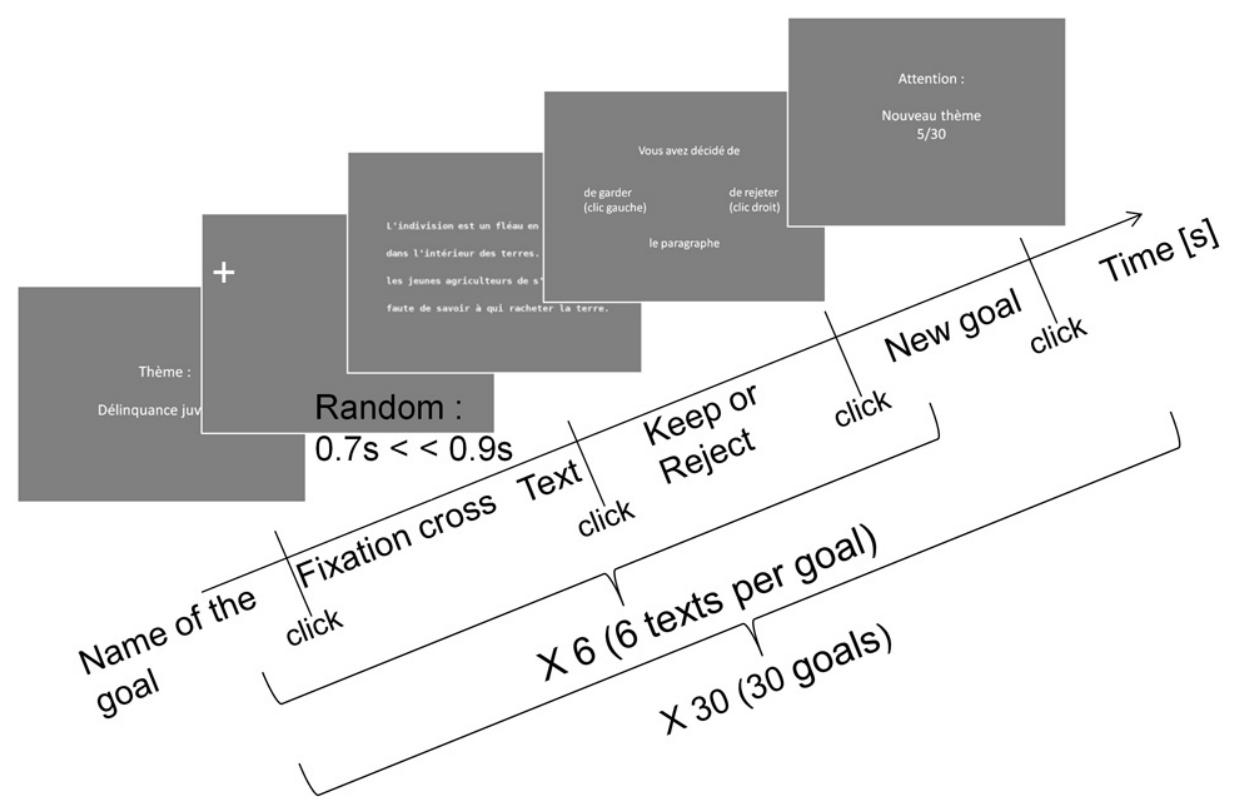
\includegraphics[width=35cm]{experiment_description.jpg}
                    \caption{Frey et al. 2013}
                \end{figure}

                \begin{itemize}
                    \item Measurements of eye positions over time and 30-channel EEG
                \end{itemize}

            \end{block}
            \vfill
            \begin{block}{Data pre-processing}
                \begin{figure}[h]
                    \centering
                    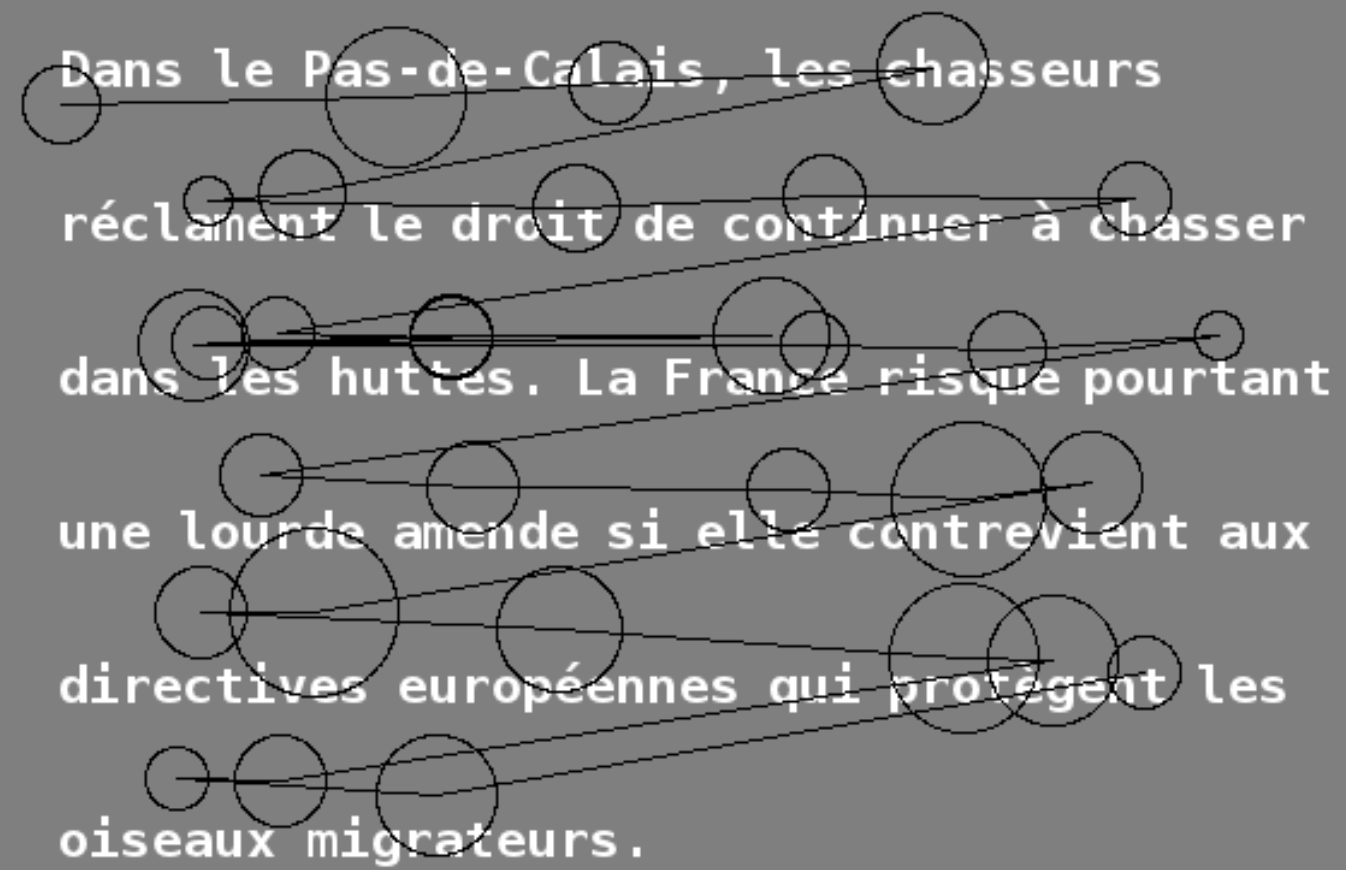
\includegraphics[width=35cm]{s4t9bl.png}
                \end{figure}
                \begin{itemize}
                    \item Scanpath : set of fixations and saccades.
                    \item Data augmentation :
                    \begin{itemize}
                        \item Participant, text, subject
                        \item Coordinates X,Y of fixations
                        \item Fixation durations, number of words between fixations
                        \item  
                    \end{itemize}
                \end{itemize}
            \end{block}
            \vfill
          }
        \end{minipage}
      \end{beamercolorbox}
    \end{column}
    % ---------------------------------------------------------%
    % end the column

    % ---------------------------------------------------------%
    % Set up a column
    \begin{column}{.49\textwidth}
      \begin{beamercolorbox}[center,wd=\textwidth]{postercolumn}
        \begin{minipage}[T]{.95\textwidth} % tweaks the width, makes a new \textwidth
          \parbox[t][\columnheight]{\textwidth}{ % must be some better way to set the the height, width and textwidth simultaneously
            % Since all columns are the same length, it is all nice and tidy.  You have to get the height empirically
            % ---------------------------------------------------------%
            % fill each column with content

            \begin{block}{References}
                \begin{enumerate}
                    \item Frey, Aline; Ionescu, Gelu; Lemaire, Benoit; López-Orozco, Francisco; Baccino, Thierry; Guérin-Dugué, Anne. 2013.
                    Decision-making in information seeking on texts: an eye-fixation-related potentials investigation.
                    \textit{Frontiers in systems neuroscience} 7 (8): 1-22

                    \item Simola, Jaana; Salojärvi, Jarkko; Kojo, Ilpo. 2008.
                    Using hidden Markov model to uncover processing states from eye movements in information search tasks
                    \textit{Cognitive Systems Research} 9 (4): 237-251

                    \item Yu, Shun-zheng. 2010.
                    Hidden semi-Markov models.
                    \textit{Artificial Intelligence} 174 (2): 215-143
                \end{enumerate}
            \end{block}
          }
          % ---------------------------------------------------------%
          % end the column
        \end{minipage}
      \end{beamercolorbox}
    \end{column}
    % ---------------------------------------------------------%
    % end the column
  \end{columns}
  \vskip1ex
  %\tiny\hfill\textcolor{ta2gray}{Created with \LaTeX \texttt{beamerposter}  \url{http://www-i6.informatik.rwth-aachen.de/~dreuw/latexbeamerposter.php}}
  %\tiny\hfill{Created with \LaTeX \texttt{beamerposter}  \url{http://www-i6.informatik.rwth-aachen.de/~dreuw/latexbeamerposter.php} \hskip1em}
\end{frame}
\end{document}


%%%%%%%%%%%%%%%%%%%%%%%%%%%%%%%%%%%%%%%%%%%%%%%%%%%%%%%%%%%%%%%%%%%%%%%%%%%%%%%%%%%%%%%%%%%%%%%%%%%%
%%% Local Variables:
%%% mode: latex
%%% TeX-PDF-mode: t
%%% End:
